\documentclass[11pt]{article}
\usepackage[utf8]{inputenc}
\usepackage[toc,page]{appendix}
\usepackage[utf8]{inputenc}

\usepackage{natbib}  %havard referencing
\bibliographystyle{agsm}
\usepackage{xcolor}
\usepackage[tikz]{bclogo}
\usepackage[framemethod=tikz]{mdframed}
\usepackage{lipsum}
\usepackage{tikz,lipsum,lmodern}
\usepackage[most]{tcolorbox}
\usepackage{caption}
\usepackage{etoolbox}
\AtBeginDocument{\patchcmd{\label}{\strut}{}{}{}}
\usepackage{amsmath}
\usepackage{amssymb}
\usepackage[ruled,vlined]{algorithm2e}
\usepackage{amsthm}
\usepackage{amsfonts}
\usepackage{graphicx}
\usepackage{amsmath}
\usepackage{amssymb}
\usepackage{amsthm}
\usepackage{amsfonts}
\usepackage{xspace}
\usepackage{mathtools}
\usepackage[noend]{algpseudocode}
\usepackage{color}
\usepackage{tikz}
\usetikzlibrary{arrows}
\usepackage{xmpmulti}

\title{Scheduling of Ticket Inspectors in Deutsche Bahn Inter-City Express Trains\footnote{This work was done when the three authors joined the G-RIPS 2019 Team at Zuse Institut Berlin,  working
on the mobile ticket inspection
project sponsored in part 
by the Deustche Bahn Railway Company. All authors contributed equally to this project.}}
\author[1]{Nathan May}
\author[2]{Hai Nguyen}
\author[3]{Ruby Abrams}
\affil[1]{Department of Mathematics,  Washington State University, U.S.A.}
\affil[2]{School of Computer Science,  University of Birmingham, U.K.}
\affil[3]{Department of Mathematics,  University of Arizona, U.S.A.}

\date{August 15, 2019}

\begin{document}
\maketitle

\begin{abstract}
add an abstract here
\end{abstract}

\tableofcontents

\section{Introduction}

\subsection{Motivations}

\par 
%A recent report from Deustche Bahn \cite{DBFactFigure2017} shows that 
%there were about $86.7$ million passengers using 
%the Inter-City Express (ICE) trains in 2017. 
Currently the staff on the ICEs 
need to stay on-board for the whole route (or most part of the route) to inspect passenger tickets. Though this ensures all passengers are checked,
the number of inspectors required scales linearly with the number of trains; otherwise, some trains
do not have any inspectors. This is a major problem with the current scheduling system because
the number of boarding and alighting passengers is generally very small compared to the 
total number of passengers currently on-board, which leads many passengers being
inspected more than once (i.e., the problem of double-counting). It may be thus more
efficient not to have the inspector staying on the same train for the entire time, but joining 
the train at some point, inspecting passengers currently on-board, and then leaving at some other
point. In this work, we try to formulate an alternative
model, where the ticket inspectors join the train 
only for a short part of the route, while maximising the number of passenger tickets inspected. 
  
\subsection{Related Work}

\citet{gao_jia_2016} describe flow of passengers in and out of trains, platforms, and stations. This specifically models pedestrian flows in a station using agent based modelling. A probabilistic variation could help determine the number of passengers boarding or alighting the train at each station.

A common technique to study the inspector scheduling problem relies on Stackelberg strategies from Game Theory \cite{osborne1994course}. This models a transportation system as a leader-follower game. In this context, the leader would be represented as the transportation system or its inspectors and the followers would be passengers. The game is played on a turn-by-turn basis, where each player (leader and follower) acts to optimise their respective objective function. These games are generally formulated as bi-level optimisation problems and implemented as Linear Programs.

An example of such an implementation is done by \citet{jiang_sandholm_2012}. Inspectors move within the Los Angeles transit system to catch fare evaders. This is also modelled as a Stackelberg strategy and stated as a bi-level optimisation problem. The leader represents inspectors, and the followers are passengers that choose to buy a ticket or not. Optimal scheduling requires temporal and spatial constraints to defer fare evasion and maximise revenue. This is also proposed as a Stackelberg problem that is formulated as an LP ``relaxation" problem.

\citet{yin_sullivan_2012} improves on the previously stated work in \cite{jiang_sandholm_2012}. This paper develops an application for randomised inspector scheduling in transit systems using leader-follower Stackelberg games whilst also maximising the expected total revenue generated from ticket sales. It studies the inspector scheduling problem in the Los Angeles metro system and addresses two main issues: complex inspector assignments and infeasible strategies. Complex inspector assignments arise when the program produces schedules for inspectors that require many train changes. This can be difficult for the inspector to remember and result in sub-optimal inspections. Infeasible strategies refer to violating the maximum number of patrol hours. Each issue is tackled by adding a sufficient amount of information to each vertex of their \textit{transition matrix} to encode history of travel for each inspector to choose the easiest route to take in the future. To do this, they develop a \textit{History-Duplicate Transition graph} (HDT). To ensure inspectors do not work more than the maximum number of working hours, sub-graphs corresponding to paths of time length less than or equal to the maximum number of working hours are embedded into the HDT. Another goal of effective randomized scheduling is to deter passengers from not buying tickets.

\citet{mastersthesis} states that the inspector scheduling problem is not a well studied problem and yet has many open areas. The author first studies the Los Angeles transit system previously considered in \cite{jiang_sandholm_2012, yin_sullivan_2012} to formulate and solve this problem as a Linear Program problem, then adapts it to solve this problem in Oslo's transit system.

A common tool used in transportation research is the Origin-Destination (OD) matrix. 
Surveying data is resource expensive, so estimating this data 
is more efficient. However, the problem
of estimating the OD matrix is still one of the most challenging problems
in transportation to date \cite{KRISHNAKUMARI2019}. More specifically, the problem is under-defined 
due to the fact that the number of independent equations that can be formulated to constraint 
OD flows with actual observations is significantly smaller than the number of OD pairs
\cite{KRISHNAKUMARI2019}.  \citet{caceres_romero_benitez_2011} proposes an 
iterated algorithm to approximate the OD matrix given
no further data other than the train schedules with passenger numbers.

A survey paper on approximating the O-D data is done by \citet{bera_krishna_rao}. This paper surveys the state-of-the-art techniques to generate such data using methods from statics to machine learning. Most techniques require prior knowledge of the transportation system or can be applied to specific scenarios.

The breakthrough work in approximating OD data was done by
\citet{van_zuylen_willumsen_1980}, where two models based on
information minimisation or entropy maximisation were developed
to predict the most likely OD matrix.
Empirical results were consistent with the data using traffic counts information 
\cite{van_zuylen_willumsen_1980}. The authors present derivation of these models that do not require any \textit{a priori} knowledge and allow for the models to encode any known information if it exists. Their section on the multi-proportional algorithm is used to develop the results in this paper.

\subsection{Our Contributions}
As already mentioned, we in this paper try to construct an alternative model to 
address the ticket inspection scheduling problem in Deutsche Bahn ICE trains, where the inspectors
do not need to stay onboard for the whole journey. Our work is different from previous work in 
\begin{enumerate}
    \item We try to maximise the number of passengers inspected by working inspectors, while previous work considers the maximisation of revenue (i.e., including 
    fine from fare evaders and ticket sales).
    \item A Stackelberg game between fare evaders and ticket inspectors has been commonly studied 
    before, we do not consider any game playing in our model, which also means that the two roles
    in our model is passengers (whether or not is fare evaders) and inspectors.
    \item Although the inspectors can inspect passengers on the trains (i.e., on-train inspection)
    or at the way out (i.e., on-station inspection), we only consider the on-train inspection.  
\end{enumerate}
Our contributions are three-fold as follows.
\begin{enumerate}
    \item  We first demonstrate how to formulate the problem of scheduling ticket inspectors 
    as a Network Flow Problem. We rigorously re-write the problem as a 
    Mixed Integer Problem (MIP).
    \item We then estimate the OD Matrix to approximate the number of 
    passengers travelling between any pair of stations. Once the number of passengers 
    of each type is obtained, general linear programming solver like 
    \textsc{Cplex} or \textsc{Gurobi} is used to solve our MIP problem.
\end{enumerate}

\subsection{Outline of Paper}
\par We end this introduction with definitions and formalised notation to use throughout the rest of the paper. Section 2 describes the different components of the mathematical model developed to solve this problem. We start with the main object of study, a multi-weighted directed graph representation of the input train schedules. Then explain how we estimate the number of passengers travelling through each path of the directed graph. Lastly, we formalize this problem as a Mixed Integer Program. Section 3 will discuss implementation and limitations of our program. We will also discuss heuristic approaches to reducing the problem size and some experiments performed to test the effectiveness of these approaches. Section 4 will discuss the complexity of this problem and discussion on issues and future research directions.

\section{Preliminaries}

In this section, we will give a deeper discussion on the considered problem, the used 
dataset and some assumptions.

\subsection{Problem Definition}

\par Given train schedules from Deutsche Bahn for various ICEs (Inter-City Express trains) and a list of train inspectors with their respective bases, produce schedules for each train inspector that maximize the total number of passenger tickets inspected throughout the day. We also account for the added restriction of bringing inspectors back to their base station at the end of their shift.

\subsection{Dataset}
\par We are given train schedules and inspector-base lists. The train schedules describe an arrival/departure event of an ICE (Inter City Express) at some time of day to/from a train station and provides information about the train ride, namely, the number of passengers on each arc and the amount of time it takes for the train to complete its journey. We have worked with the ICE 1 for a particular Monday. Schedules for other trains on other days can be developed in the same way. The inspector-base list comprises of the ``inspector resources". It is a list of base stations and the number of of inspectors that are based out of each station.

\begin{figure}[t]
    \centering
    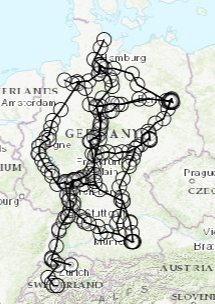
\includegraphics[scale=0.7]{pics/GermanyTrainMap.png}
    \caption{A map of Germany and Switzerland depicting all train stations as circles and train routes as lines between stations for the Deutsche Bahn.}
    \label{fig:map}
\end{figure}

% =====================================
% This section may be omitted
% =====================================
% it is used to motivate the use of developing O-D matrices and was a natural step in the progression of our research 
\par The naive approach considers train inspectors maximizing the number of tickets inspected on each train ride. However, this is not an efficient approach since passengers generally travel on trains for multiple stops. This naive approach would push passengers to be inspected multiple times. So we need to develop methods for keeping track of the number of passengers on each train ride that have been inspected.

\subsection{Assumptions and Simplifications}

We list assumptions in our model and follow each with how they were used.

\begin{assump}
All inspectors inspect at the same rate.
\end{assump}
This was used to compute the \textit{arc effectiveness} for each inspector. Different inspection rates may be easily incorporated into the model, but may be difficult to acquire as input data.

\begin{assump}
All paths taken are the shortest paths.
\end{assump}
This is a redundant assumption, because all passengers (no matter the path) will travel along the directed graph and have some start and end time (and cannot go back in time). However, it will be necessary for explaining the structure of the diagonal of the Origin-Destination matrix.

\begin{assump}
Not every inspector has to work.
\end{assump}
Given all inspector resources, it may not be necessary to solve this problem using all inspectors. It should be sufficient to use some subset of inspectors that ``sufficiently" span the network and inspect some minimum percentage of passengers traveling throughout the day.
\begin{assump}
    Every arc in our graph is unique.
\end{assump}
Our data suggests that multiple disjoint trains can travel between the same two stations at the same time. i.e. Inspectors cannot transfer between these trains. We can accommodate for this case by:
        \begin{itemize}
            \item[(1)] Storing multiple arcs using a Multi-DiGraph structure.
            \item[(2)] Modifying the multi-proportional algorithm to account for multiple shortest paths in the Origin-Destination Matrix. 
        \end{itemize}
         This may be direction for further development.
\begin{assump}
    Our data set it complete.
\end{assump}
This is used for estimating the Origin-Destination matrix. No additional information is provided about passengers information other than passenger counts on each train ride. Since we lack information about number of passengers that wait at a station for their next train, passengers who layover at a station before catching the next train will be counted as two different passengers.

\begin{assump}
     Inspectors working the maximum number of working hours will optimize the objective function.
\end{assump}
We use this in implementation. 
The greedy approach is used to reduce the problem instance to a smaller pool inspectors to choose from. 


\section{Mathematical model}

\subsection{Notation}
\begin{itemize}\itemsep -2pt
    \item $G = (N,E)$ is our graph with nodes and arcs
    \item $N = \{$nodes in the graph without sinks or sources$\}$
    \item $n = ($station , event$)\quad \forall n\in N$
    \item $E = \{$arcs/arcs$\}$
    \item $K = \{$inspectors$\}$
    \item $\Lambda\subset\mathcal{P}(N)$ is the set of all paths
    \item $\delta^+(B) = \{$out going arcs of node $B\}$. i.e. the \textit{predecessors} of $B$
    \item $\delta^-(B) = \{$incoming arcs of node $B\}$. i.e. the \textit{successors} of $B$
    \item $S_k$ is the source node of the $k^{th}$ inspector
    \item $T_k$ is the sink node of the $k^{th}$ inspector
\end{itemize}


% We want to maximize the probability that an uninspected passenger from a previous trip is inspected before that passenger arrives to their destination.



\subsection{Graph Representation}

The main object of study is the directed graph (which is a network flow) representing the flow of trains and passengers throughout the day. 
The nodes of the graph represent \textit{events}, where each event is either an \textit{arrival} or \textit{departure} of a train into or out of a station. Each node is then uniquely identified by a space-time pair, the station and time of event. 
Each arc represents a train ride from a departure station at a starting time to an arrival station at an ending time. This is used to distinguish between multiple trains rides using the same tracks. We incorporate the time of day that a train arrives or departs to induce an acyclic flow through the graph. 

Each arc has associated information extracted from the input train schedule data that describes the train ride taken on that day: (a) the number of passengers on each train ride, $v_e$ and (b) the amount of time taken from departure to arrival, $t_e$. An associated binary variable, $x_e^{(k)}$, also known as a decision variable, is also associated to each arc. If $x_e^{(k)} = 1$, then the $k^{th}$ inspector takes arc $e$, otherwise, not. This variable is the output of a linear program. See Figure \ref{fig:arc} for a graphical description of each arc.

Every passenger trajectory is assumed to be the shortest path taken and can be determined (not uniquely, as multiple shortest paths could exist) as a pair of nodes starting station and start time and ending station and end time. See Figure \ref{fig:passenger_path} for an example passenger path.
\begin{figure}
    \centering
    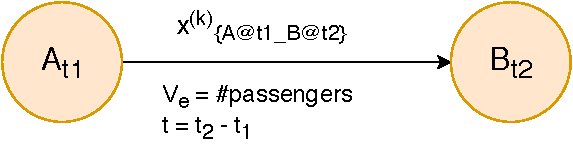
\includegraphics[scale=0.7]{pics/nodes.pdf}
    \caption{Description of an arc between nodes and properties associated to each}
    \label{fig:arc}
\end{figure}

\begin{figure}
    \centering
    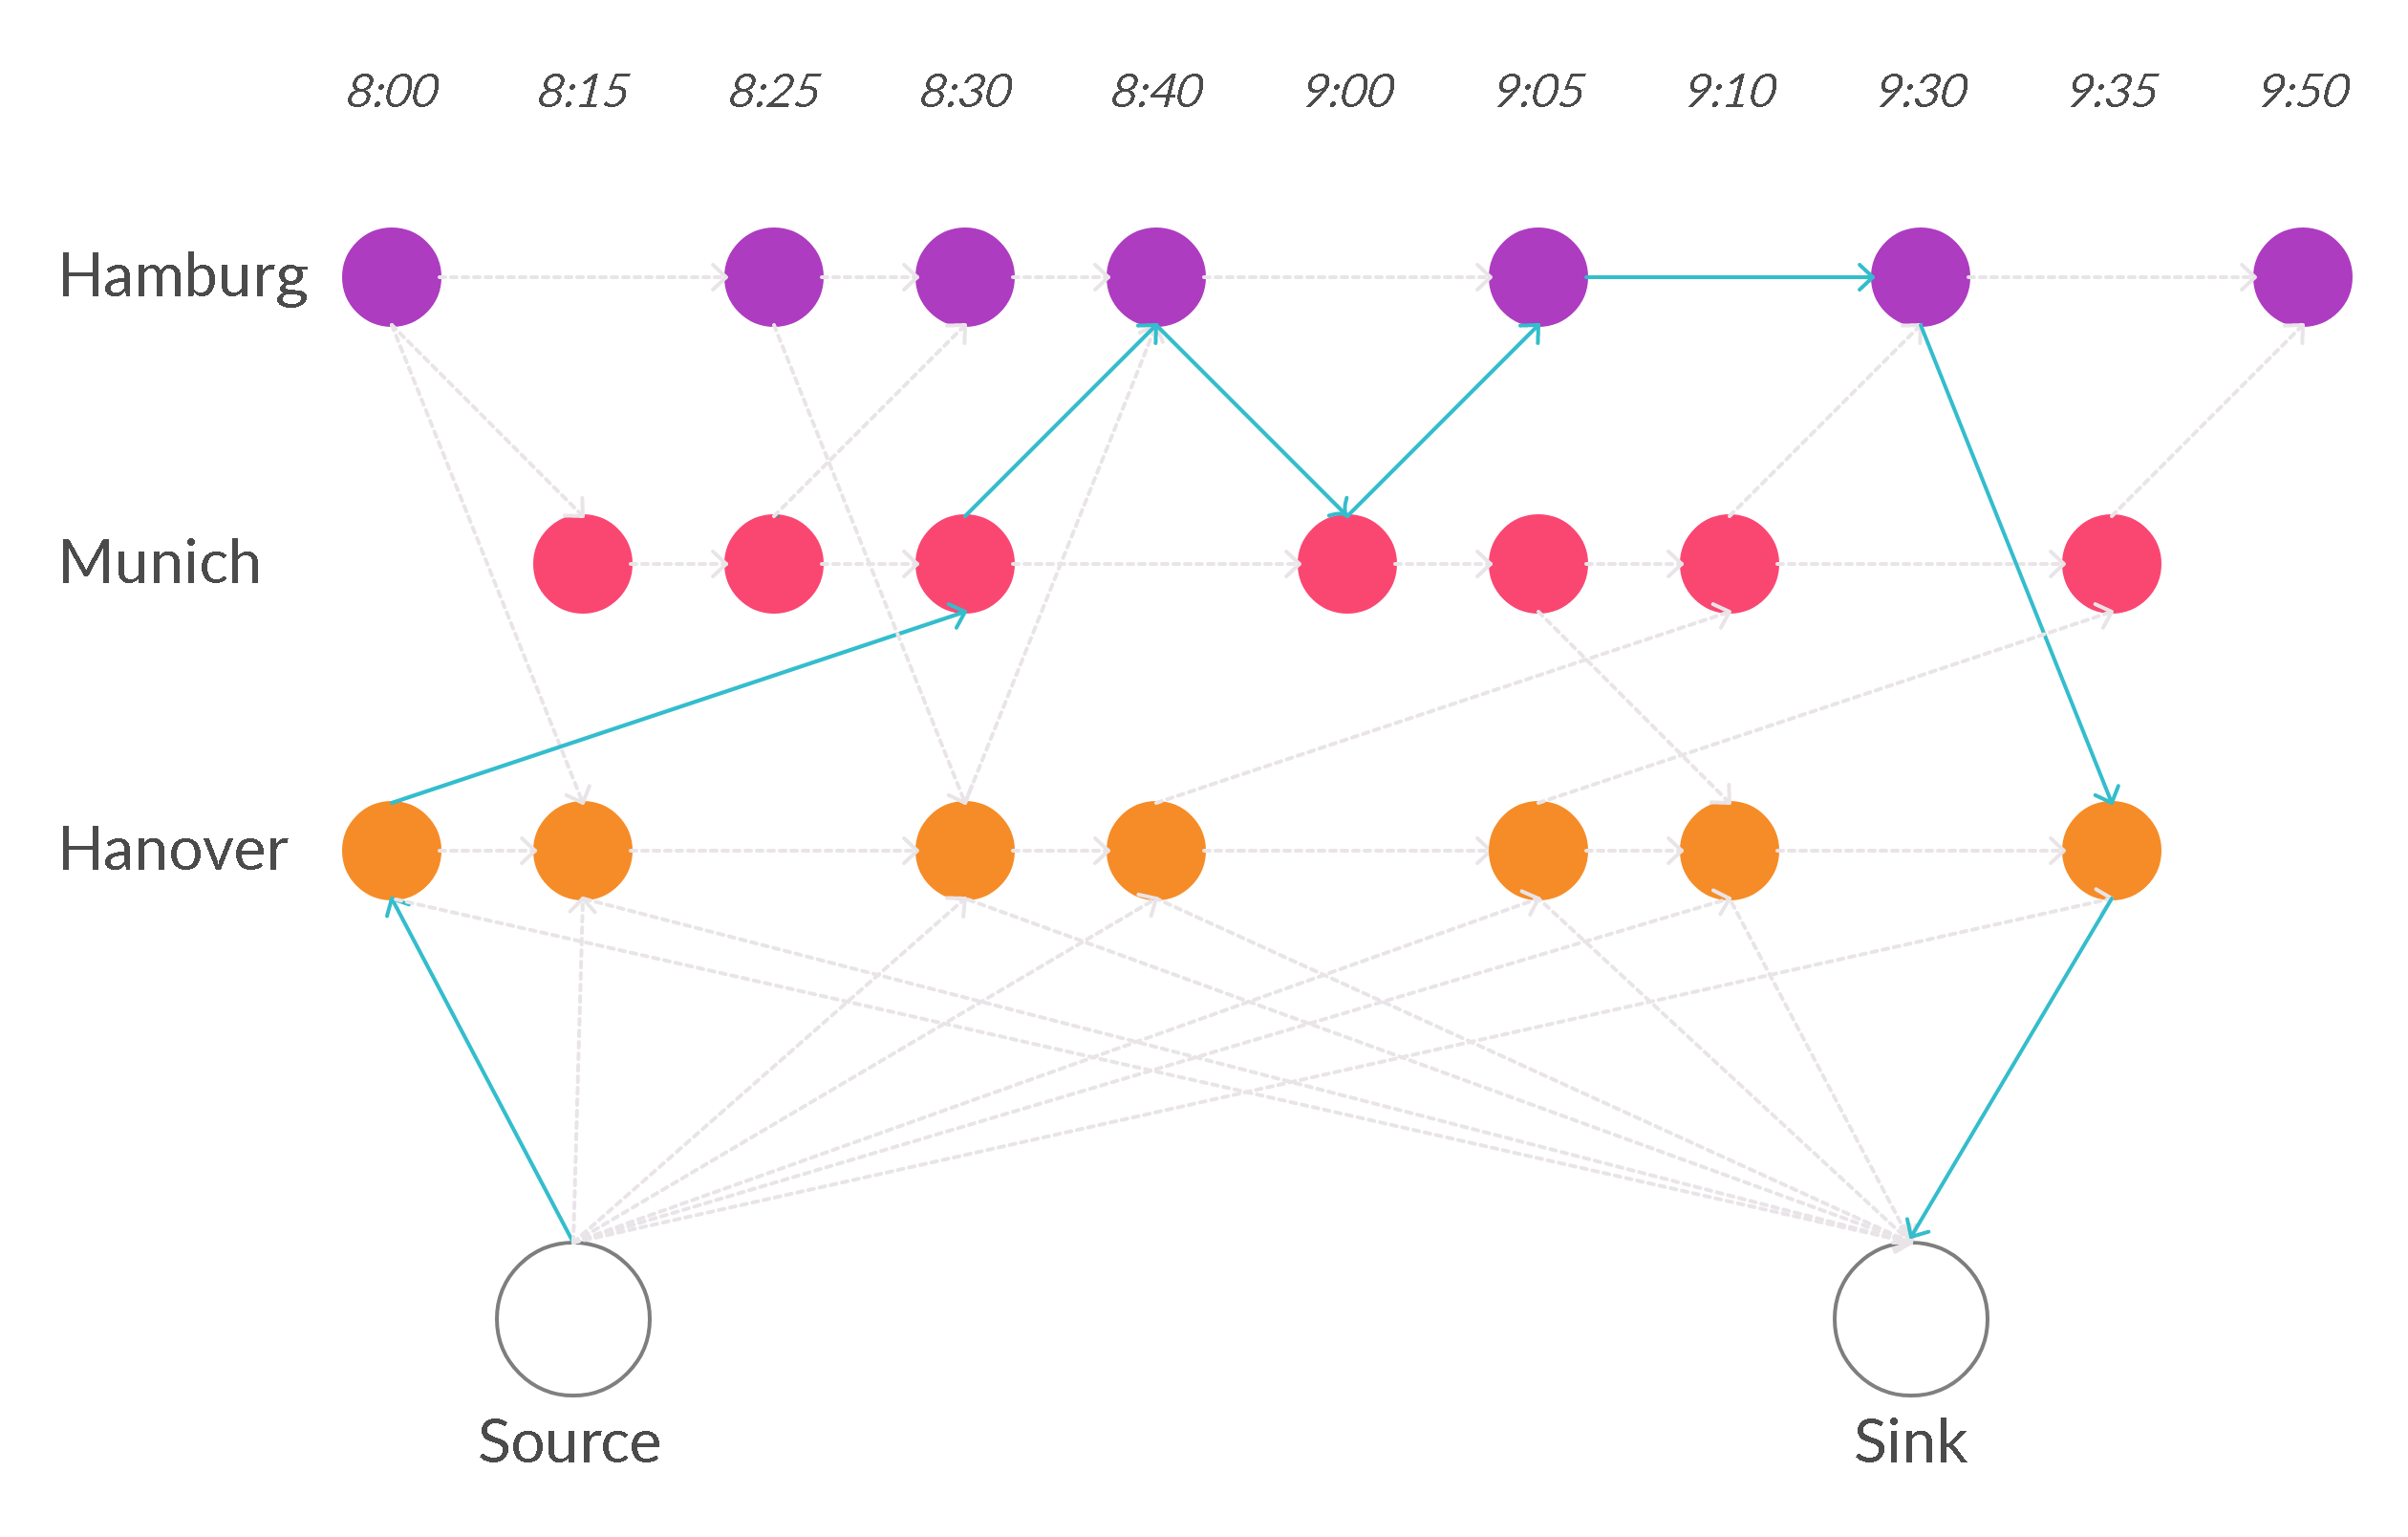
\includegraphics[scale=.15]{pics/Inspector_Path_Example.jpg}
    \caption{An example trajectory for an inspector is highlighted in blue starting at the Hanover station at 8:00 am and ending at the Hanover station at 9:35 am. Dummy nodes known as source and sink are also attached.}
    \label{fig:patrol_strategy}
\end{figure}

The network flow graph can be represented by two axes: the train station name and time events (where each event is an arrival or departure of some train). arcs in this graph are classified as either \textit{driving} (train changing stations) (Figure \ref{fig:driving_arcs}) or \textit{waiting} arcs (train staying at the same station) (Figure \ref{fig:waiting_arcs}). An example network flow graph is depicted in (Figure \ref{fig:graph}). We solve the inspector scheduling problem for each inspector. This means for $|K|$ inspectors, there are $|K|$ unknown decision variables associated to each arc in the graph. i.e. a binary-valued vector of length $|K|$ is associated to each of the graph and is the output of our Linear Program.

Each inspector is required to start and end at the same station. To impose this constraint, we attach ``dummy" nodes called a \textit{source} and \textit{sink} nodes. These nodes are connected to every node of the inspector's base station. This will allow the output of the program to determine where in the graph the inspectors need to start and end. See Figure \ref{fig:sink_and_source}. An example inspector trajectory is depicted in Figure \ref{fig:patrol_strategy}.
\begin{figure}
    \centering
    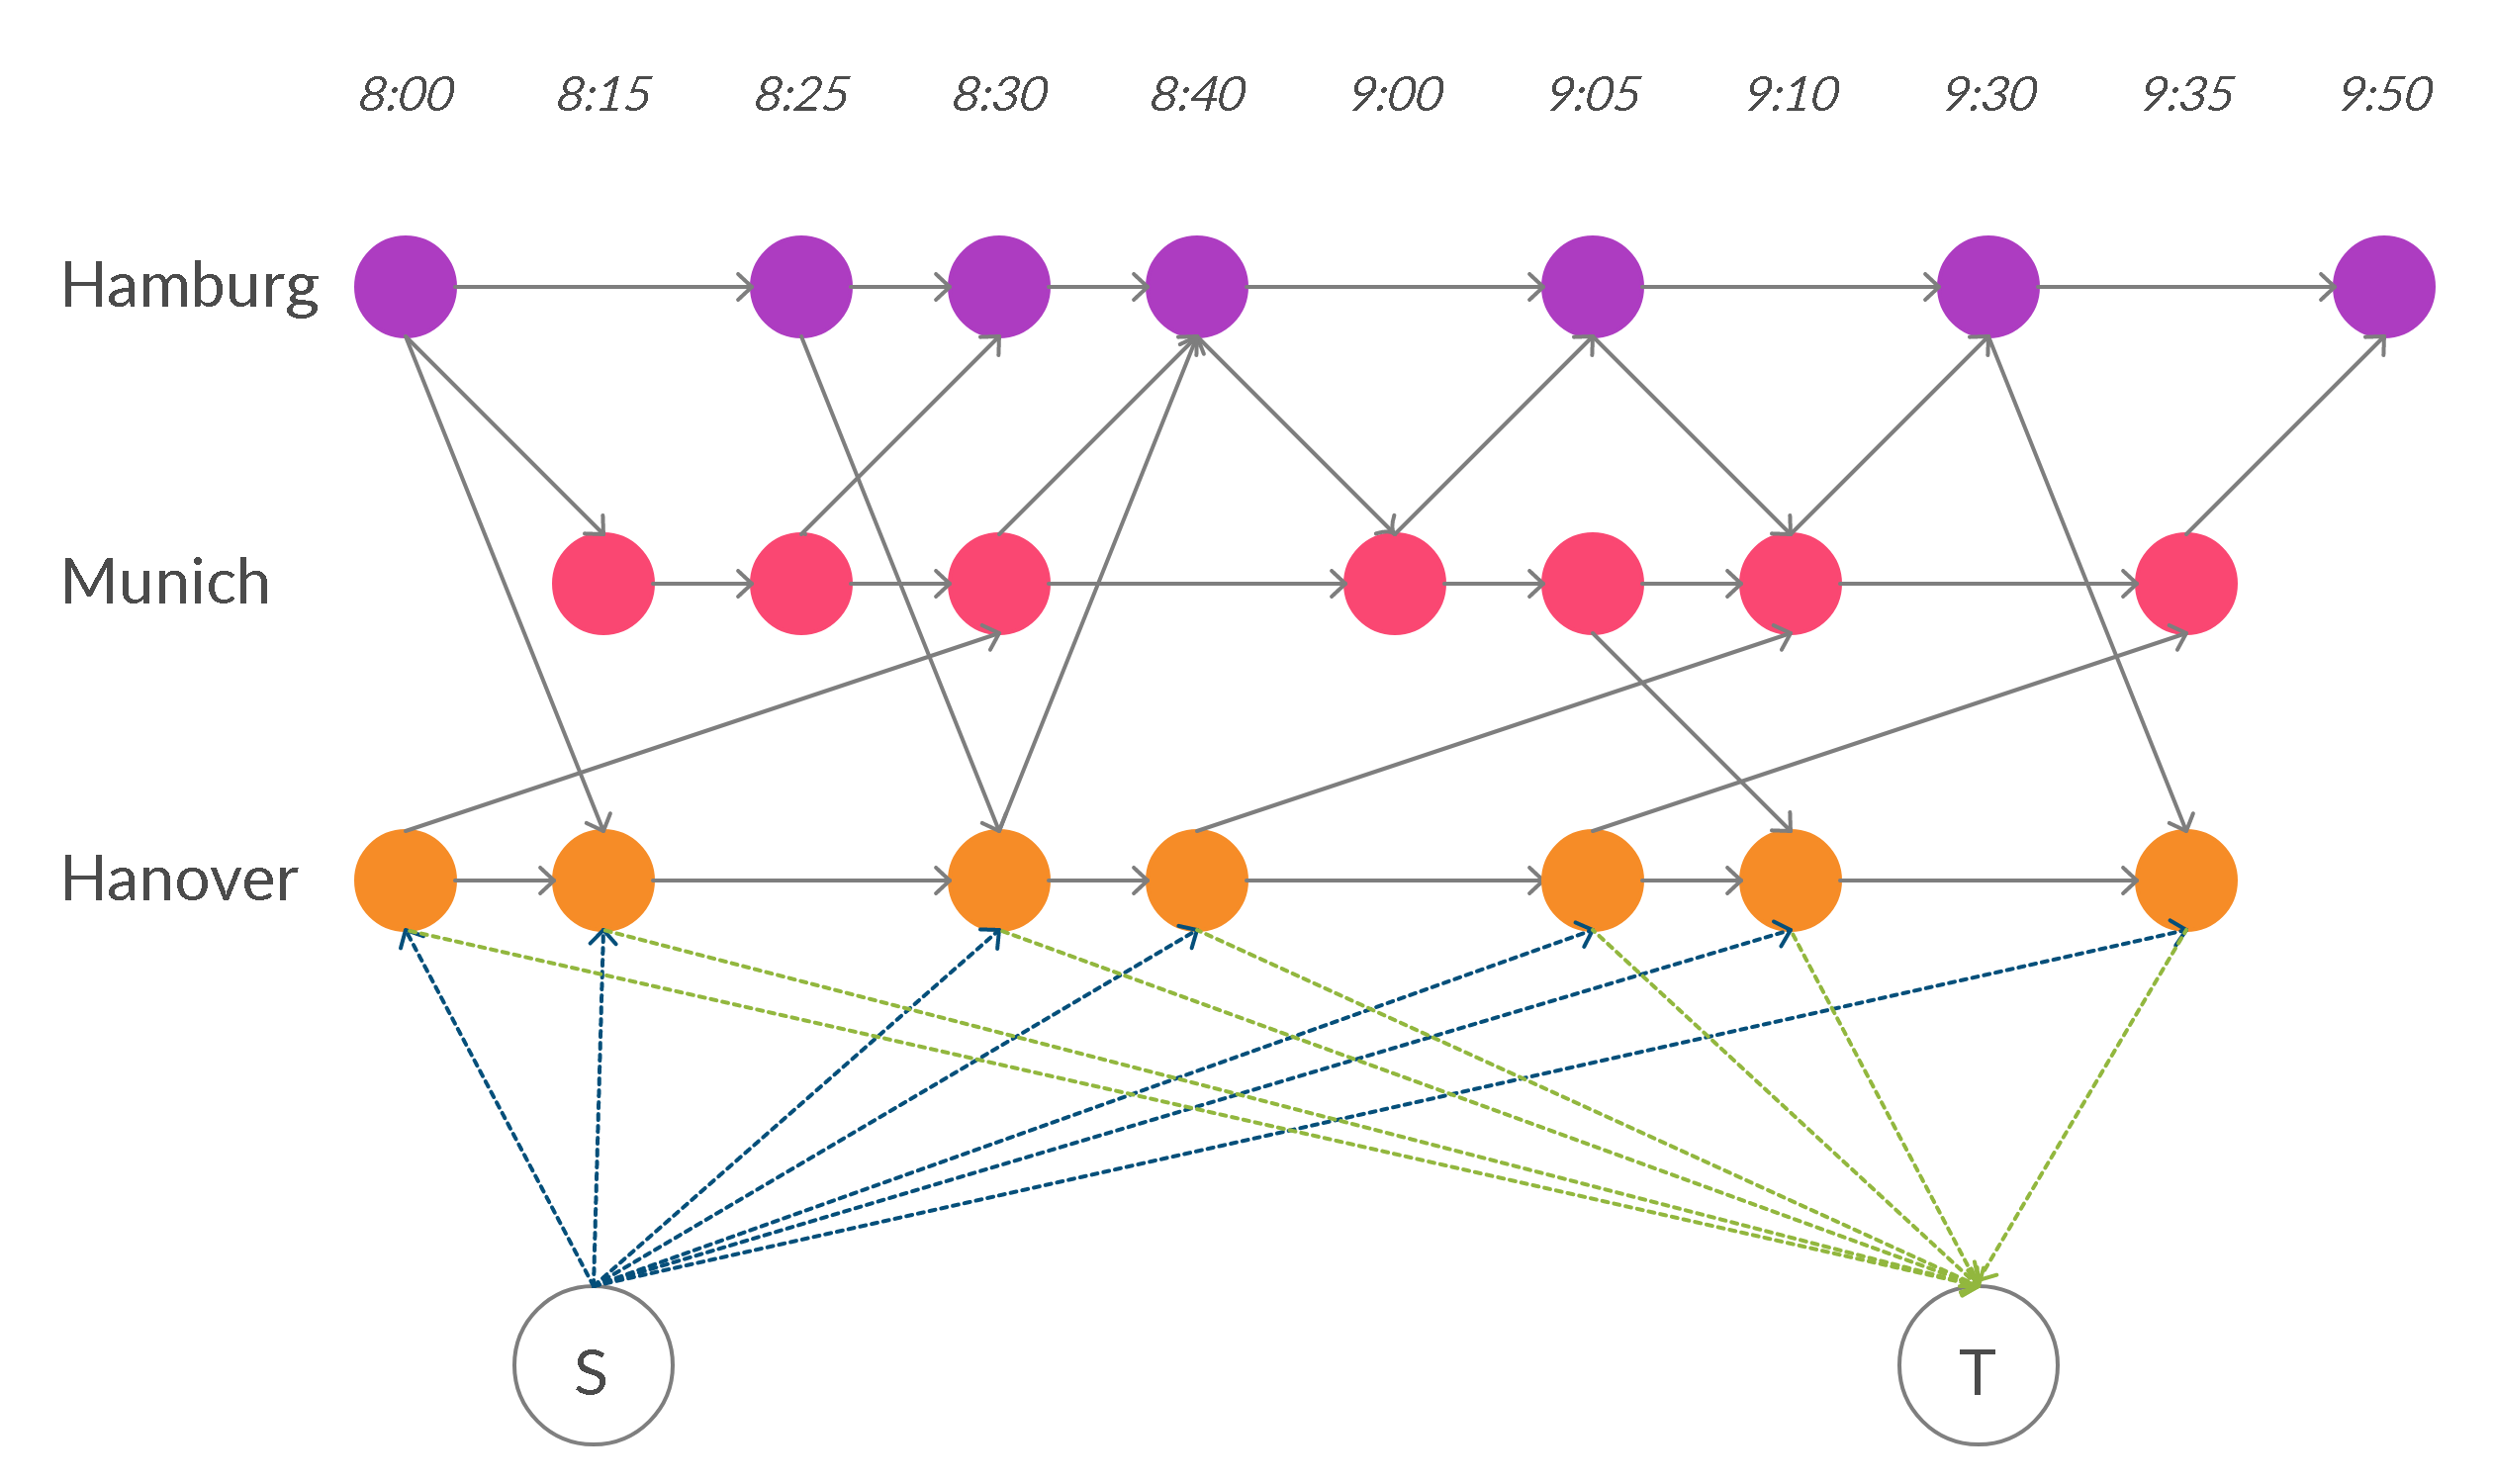
\includegraphics[scale=0.15]{pics/Graph.jpg}
    \caption{Simple example of a network flow graph with 3 base stations (stations Hamburg, Munich, and Hanover) and discretized temporal events (arrival/departure). A sink and source node are attached to all possible nodes of the station at Hanover.}
    \label{fig:graph}
\end{figure}
\subsection{Origin-Destination Matrix}
\par The Origin-Destination (OD) matrix is useful in urban transportation design and planning, but difficult to information to acquire. \citet{bera_krishna_rao} give a brief over view of the different methods, like bi-level programming and machine learning, to estimate the OD matrix. However, most of these approaches assume a priori knowledge acquired via sampling. Since we do not assume any a priori knowledge about the system, the most appropriate method to use is the original paper by \citet{van_zuylen_willumsen_1980}, which proposes a maximum entropy/information minimisation  approach to computing the OD matrix. We refer to the multi-proportional algorithm in their paper for details on implementation. The input of this algorithm is the directed graph with the volume counts (the number of passengers on each arc) and the output of the algorithm is a matrix whose $(i,j)$ entry represents the number of people who travelling from starting node $i$ to ending node $j$.


\subsection{The Mixed Integer Program}

\subsubsection{Probability of passenger inspection}

According to \cite{jiang_sandholm_2012, mastersthesis, yin_sullivan_2012}, we can quantify the probability that a certain passenger type is inspected. It is defined by
\begin{align}
    \min\bigg\{1,\sum_{i=1}^\gamma\sum_{e\in P_i\cap\lambda} f_e\bigg\}
\end{align}
where $f_e$ is the \textit{arc effectiveness} value of a patrol unit on arc $e$, $\gamma$ is the number of deployable patrol units, $P_i$ is the $i^{th}$ patrol strategy (a path subset of the graph), and $\lambda$ is a passenger type (also a path subset of the graph). The arc effectiveness value is defined by $f_e = r\cdot t_e/v_e$, where $r\cdot t_e$ is the potential number of passengers an inspector can inspect and $v_e$ is the total number of passengers on a train ride. The inspection rate $r$ is assumed to be constant for every inspector. Thus, $f_e$ has physical interpretation of volume fraction of passengers inspected of arc $e$. Since multiple inspectors are allowed on each train ride, passengers can be inspected by portioning off sections of the train amongst the available inspectors, so that the arc effectiveness becomes additive. A passenger of \textit{type} $\lambda$ is a passenger that travels the path $\lambda$ (an ordered sequence of arcs in the directed graph).

\subsubsection{Objective as number of passenger inspected}

We formulate our objective function in the following way.

\begin{equation}
\label{objectivefxn}
     \max_{\textbf{x}}\sum_{\lambda}\underbrace{T_{\lambda}\cdot\min\bigg\{\sum_{e\in\lambda}f_e\left(
        \sum_{k=1}^K x_{e}^{(k)}
    \right), 1\bigg\}}_{\text{Expected number of passengers of type $\lambda$ inspected}}
\end{equation}
where $T_\lambda$ is the number of passengers travelling through path $\lambda$. This can be interpreted as maximising the proportion of people of each passenger type inspected, where
the value inside the sum can be interpreted as the expected number of 
passengers of type $\lambda$ being inspected.

\subsubsection{Our mixed integer programme}

We establish below the input parameters and output variables of 
our Linear Program and follow it with the completely formulated problem. 
We use \textsc{Gurobi} solvers written in Python to implement this program.

\textbf{Parameters:}
\begin{itemize}\itemsep -2pt
    \item $T_\lambda$: the number of passengers on path $\lambda\in\Lambda$
    \item $t_{(S_k,A)}$: the potential starting time stamp at node $A$ for inspector $k$
    \item $t_{(A,T_k)}$: the potential ending time stamp at node $A$ for inspector $k$
    \item $f_e$: the fraction of passengers inspected by a single inspector on arc $e$
    \item $\theta_k$: the maximum number of working hours for inspector $k$
    \item $\kappa$: the maximum number of inspectors allowed to work.
\end{itemize}

\textbf{Variables:}
\begin{itemize}\itemsep -2pt
    \item $x_e^{(k)}\in\{0,1\}$: decision variable for if inspector $k$ uses arc $e$.
    \item $\Pi_\lambda\in [0,1]$: the probability that a passenger of type (or path) $\lambda$ being inspected.
\end{itemize}

Below is the complete problem: 
\begin{equation}
    \max_{\textbf{x}} \sum_{\lambda\in\Lambda}T_\lambda\cdot \Pi_\lambda
\end{equation}
\textbf{subject to:}
\begin{align}
\begin{split}\label{mass-balance}
     \sum_{e\in\delta^+(B)}x_e^{(k)} - \sum_{e\in\delta^-(B)}x_e^{(k)} &= 0, \forall B\in N, \forall k\in K\\
\end{split}\\
\begin{split}\label{source}
         \sum_{e\in\delta^+(S_k)}x_e^{(k)}
         \le 1, \forall k\in K\\
\end{split}\\
\begin{split}\label{time-flow}
          \sum_{e\in\delta^-(T_k)}x_e^{(k)}\cdot t_e - \sum_{e\in\delta^+(S_k)}x_e^{(k)}\cdot t_e 
          \le \theta_k, \forall k\in K\\
\end{split}\\
\begin{split}\label{minimum}
        \Pi_\lambda 
        \le \sum_{\substack{e\in\lambda k \in K}}f_e\cdot x_e^{(k)}, \forall\lambda\in\Lambda\\
\end{split}\\
\begin{split}\label{max_num_insps}
        \sum_{k\in K} \sum_{e\in\delta^+(S_k)}x_e^{(k)}
        \le \kappa\\
\end{split}
\end{align}

Equation (\ref{mass-balance}) represents the \textit{mass-balance} or \textit{flow conservation} constraint. This states that the number of outgoing arcs and number of incoming arcs for every node that is not a source or sink are equal.

The \textit{source constraint}, in equation (\ref{source}), is sufficient to guarantee that \textit{if} an inspector leaves a source, it will also enter a sink. This constraint with the mass-balance constraint ensures that if an inspector leaves a station from a source node, he/she will also return to that station at a sink node. The less than or equal to sign allows inspectors not to work, since it may be the case that not all resources are necessary to ensure that sufficiently many passengers are inspected.

The \textit{time flow} (or \textit{max work shift}) constraint, equation (\ref{time-flow}), imposes work schedule restriction stating that the $k^{th}$ inspector cannot work more than $\theta_k$ hours. This constraint may also be implemented as the sum of times across all arcs in the graph. The following reformulation of the time-flow constraint may speed up computation time.
\begin{align}
    \sum_{e\in E}x_e^{(k)}\cdot t_e\le \theta_k\qquad\qquad\forall k\in K
\end{align}

We impose the \textit{minimisation constraint}, equation (\ref{minimum}), because the original objective function, equation (\ref{objectivefxn}), is not a linear function, but a piece-wise linear function. To over come this, we create a new dummy variable $\Pi_\lambda$ to replace the minimum function in the objective function and impose upper bounds of its entries in as constraints. Note that $\Pi_\lambda$ has physical interpretation as the probability that a passenger of type $\lambda$ being inspected. This quantity is bounded above by $1$ and must also be less than the total inspection effectiveness of all inspectors travelling through any path.

Lastly, we used equation (\ref{max_num_insps}) for development purposes. We test our schedule building algorithm for each $\kappa\in\mathbb{N}$ and record approximate percentage of people inspected in the entire system. This imposes a maximum number of inspectors allowed to work on a given day.

\subsection{Complexity Analysis}
According to Gary and Johnson's book, \textit{Computers and Intractability: A Theory of NP-Completeness}\cite{Garey:1990:CIG:574848}, Integer Programming (IP) problems are NP-Complete in the strong sense. Thus, we encounter exponential growth of run time with respect to the size of our input. The rest of our research relies in practical implementation: creating good results in a reasonable runtime.

For each inspector, the number of unknown output variables $x_e$ is equal to the number of arcs in the directed graph. In order to determine the complexity, we need to turn our problem into an instance of an already known hard problem to conclude that our problem is at least as hard as the known hard problem. We classify our problem as a constrained shortest path problem. Further work entails reducing our problem into one of these to determine complexity. According to the appendices of \cite{Garey:1990:CIG:574848}, our problem is most similar to the following problems
\begin{itemize}
    \item Path Constrained Network Flow: $\mathcal{NP}$-Complete
    \item Vertex Covering (or restated arc Covering): 
    Vertex covering is an $\mathcal{NP}$-Complete problem.  
    Arc covering can be solved in polynomial time using graph matching.
    \item Minimum Covering: $\mathcal{NP}$-Complete, but can become solvable in polynomial time under a specific assumption. 
\end{itemize}

\section{Implementation}

\subsection{Heuristic Solvers}
We conjecture that our MIP problem is in 
$\mathcal{NP}$-class, which also means the running time will increase exponentially with 
respect to the number of inspectors. As can be seen latter that it takes 1.5 hours to
obtain the inspection schedule for 30 inspectors with an optimality gap of 5\%. The
Deutsche Bahn railway company has over 500 inspectors for the ICE 401 fleet, and solving the MIP programme for all of them simultaneously turns out to be impractical. 
Our approach to solve this problem heuristically is implementing a \textit{local search}. We reduce the number of dimensions of the problem by fixing trajectories for certain inspectors using the \texttt{useSolution()} and \texttt{setSolution()} functions from Gurobi solvers. We apply a greedy heuristic: inspectors working the maximum number of hours will contribute the most to maximizing the objective function (refer to the assumptions section). Out of the choices of inspectors to choose from, we reduce the pool of candidates to choose from to the inspectors who work the maximum number of working hours. The remaining inspectors' trajectories are set to $0$ and the problem is solved on a smaller set of unknown variables. Algorithm~\ref{algor:heuristic-solver} gives a full
description of our proposed heuristic solver for large-scale problem.

However, we encounter the following limitation of the Gurobi solver. When the inspector scheduling problem is solved for 1 inspector, a solution is obtained less than 1 second (see Table \ref{tab:runtime-without-heuristic}). When the problem is solved for 6 inspectors and the solutions for 5 of them are fixed (leaving 1 free inspector schedule to be determined), a solution is obtained in 70 seconds. Thus, our heuristic solver is the following: given a list of $I$ inspectors, where we seek to build schedules for the best $n\le I$ inspectors, we build the schedules incrementally with $\Delta$ number of inspectors at a time. By specifying $I, n$ and $\Delta$, we can build inspector schedules in a reasonable run-time. 


\begin{algorithm}[t]
    \DontPrintSemicolon
    Choose a subset of inspectors from the inspector pool\;
    \Repeat{termination condition is fulfilled}{
       Solve the current MIP model\;
       Fix the solutions for these inpsectors\;
       Add more inspectors into the model\;
    }
    \caption{Heuristic solver for large-scale problem}
    \label{algor:heuristic-solver}
\end{algorithm}

\section{Empirical results}

\subsection{Estimation of O-D Matrix}
\par We plotted the sparse OD matrix (See Figure \ref{fig:a} and \ref{fig:b}). A larger intensity of blue entries represent higher numbers of passengers of that type. We expect that no passengers are travelling from a station to itself. However, we can see a thick diagonal. We attribute the thick diagonal (even though actual diagonal entries are $0$) to the lack of \textit{waiting arc} data (see Figure \ref{fig:waiting_arcs} for visual reference). True passenger trajectories may require passengers to have a layover or ``wait" at a station before they catch their next trip. Since our algorithm does not contain any information about the number of passengers who wait at each station, these passengers are double counted. i.e. they are counted as passengers of more than one type. Since the sum of all entries in the OD matrix represent the number of people travelling throughout the system in one day, we can conclude that this number is an overestimate. This can be direction for further implementation. The multiproportional algorithm can easily be recalculated on a directed graph that contains waiting arc information (number of passengers waiting at a station).

\begin{figure}[htp]
    \centering
    \subfloat{%
     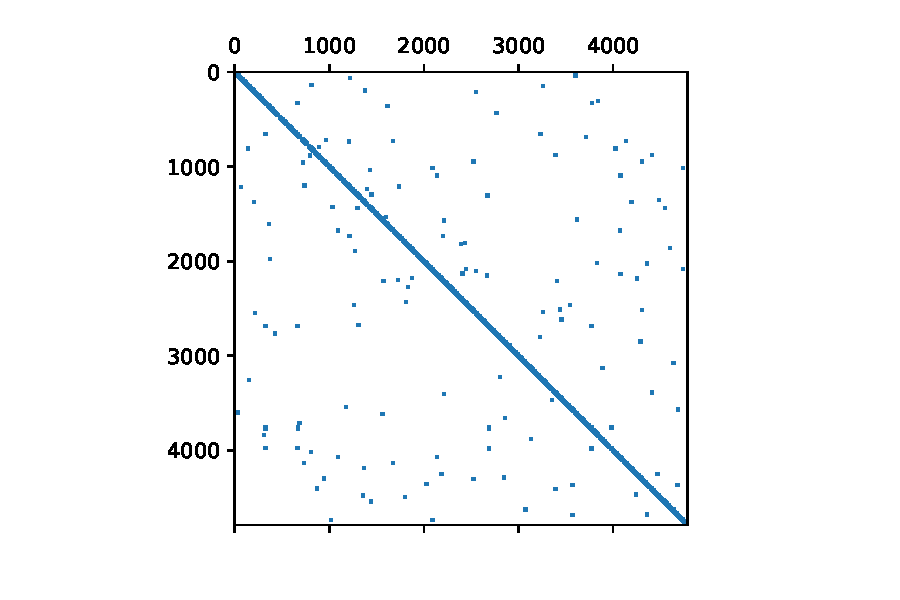
\includegraphics[scale=0.4]{pics/OD_sparse_matrix.pdf}        
     \label{fig:a}%
        }%
    \hfill%
    \subfloat{%
        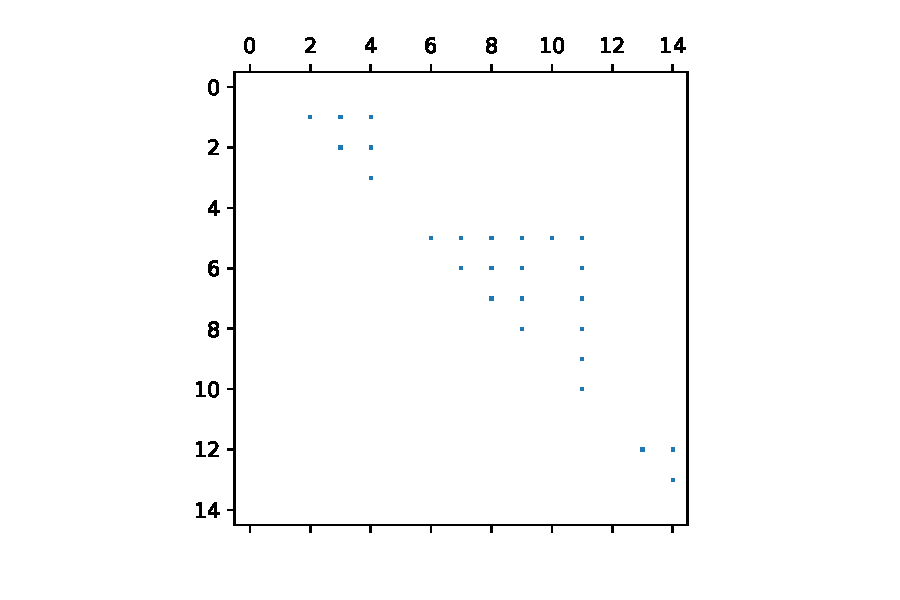
\includegraphics[scale=0.4]{pics/zoomed_in_sparse_matrix.pdf}
        \label{fig:b}%
        }%
    \caption{\textbf{Left}: Approximately 5000 nodes (events) are in our graph. The diagonal entries represent number of people travailing from one node to itself. The thick diagonal is explained by lack of waiting arc data. i.e. Passengers who layover at a station are counted twice (as part of two different paths). \textbf{Right}: A zoomed in version of the left matrix. There are no entries on the diagonal since one cannot travel by train from a node to itself. Nodes near the diagonal represents passengers travelling between nearby nodes. i.e. Many single edge rides taken.}
\end{figure}

\subsection{Solving without using heuristic solver}

\par We run some experiment to show how the 
running time scales with the 
size of the problem (i.e. number of inspectors). In this 
experiment\footnote{On MacBook Pro ver. 2017, 3.3 GHz Intel Core i5, 8 GB RAM.}, we used the 
timetable of the ICE train 401 on Monday. The time-expanded graph consists of 3593
driving arcs and 4667 waiting arcs. There are 157 stations involved in the train schedule on
this particular day. The programme also took about 18.66 seconds to  estimate the OD matrix.

We are interested in the CPU/Wallclock time taken by the programme until the optimal schedule for all inspectors is obtained. We also set the gap tolerance (called MIPGAP) of the Gurobi Solver to 10\% and 5\%.
Running time results are shown in Figure~\ref{tab:runtime-without-heuristic}. 

\begin{table}[]
\centering
\begin{tabular}{|c|c|c|c|c|}
\hline
\multicolumn{2}{|c|}{\#Inspectors} & \multicolumn{2}{l|}{CPU/Wallclock time (in seconds)} \\ \cline{3-4} 
 \multicolumn{2}{|c|}{}  & MIPGAP 5\%           & MIPGAP 10\%           \\ \hline
\multicolumn{2}{|l|}{1 (1 Depot)} & $< 1$                & $< 1$                   \\ \hline
\multicolumn{2}{|l|}{2 (2 Depots)}  & $9$                 &  $4$           \\ \hline
\multicolumn{2}{|l|}{4 (4 Depots)}  & $39$                 &  $24$           \\ \hline
\multicolumn{2}{|l|}{6 (4 Depots)}  & $36$                 &  $30$           \\ \hline
\multicolumn{2}{|l|}{10 (7 Depots)}  & $300$                 &  $104$           \\ \hline
\multicolumn{2}{|l|}{15 (10 Depots)}  & $505$                 &  $160$           \\ \hline
\multicolumn{2}{|l|}{30 (10 Depots)}  & $5617$                 &  $976$           \\ \hline
\end{tabular}
\caption{Empirical running time for different set of inspectors.}
\label{tab:runtime-without-heuristic}
\end{table}

\subsection{Solving using heuristic solver}




\section{Conclusion and Future Work}
% \section{Appendix}
% \subsection{Visual representation of components of the network}
% \begin{appendix}

% \begin{figure}
%     \centering
%     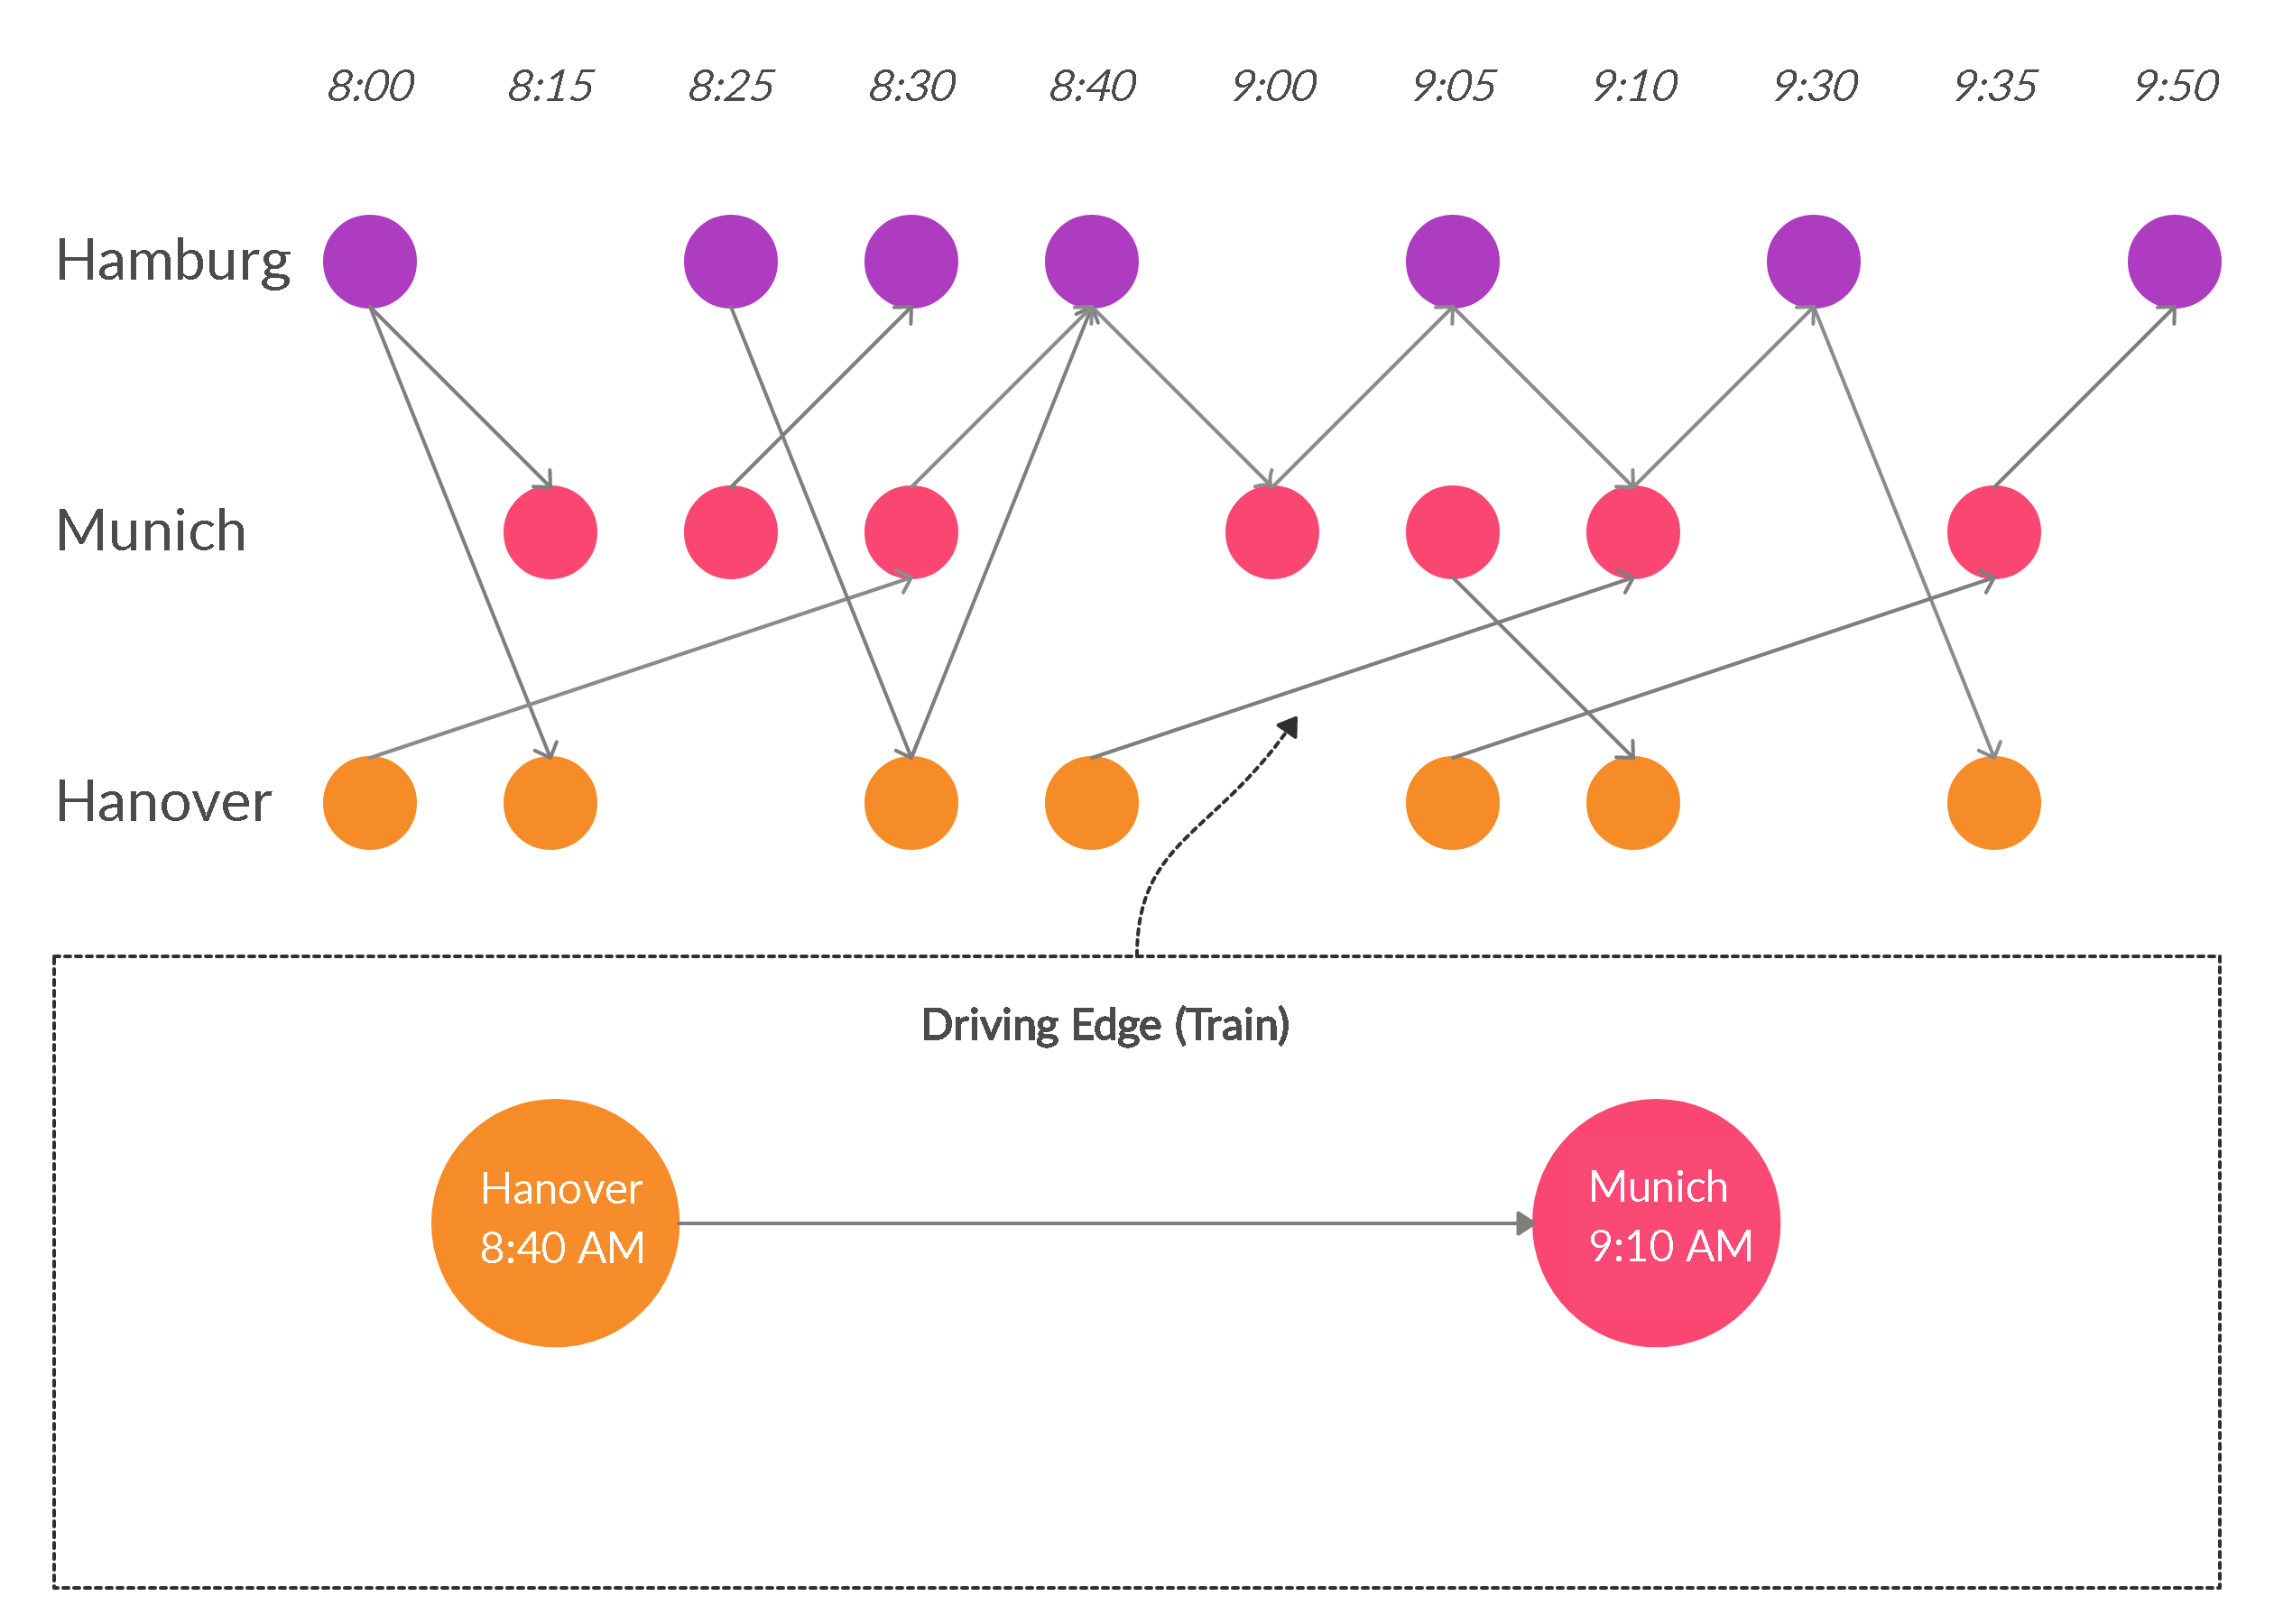
\includegraphics[scale=.15]{pics/Driving_Edges.jpg}
%     \caption{Example directed graph depicting \textit{driving arcs}}
%     \label{fig:driving_arcs}
% \end{figure}
% \begin{figure}
%     \centering
%     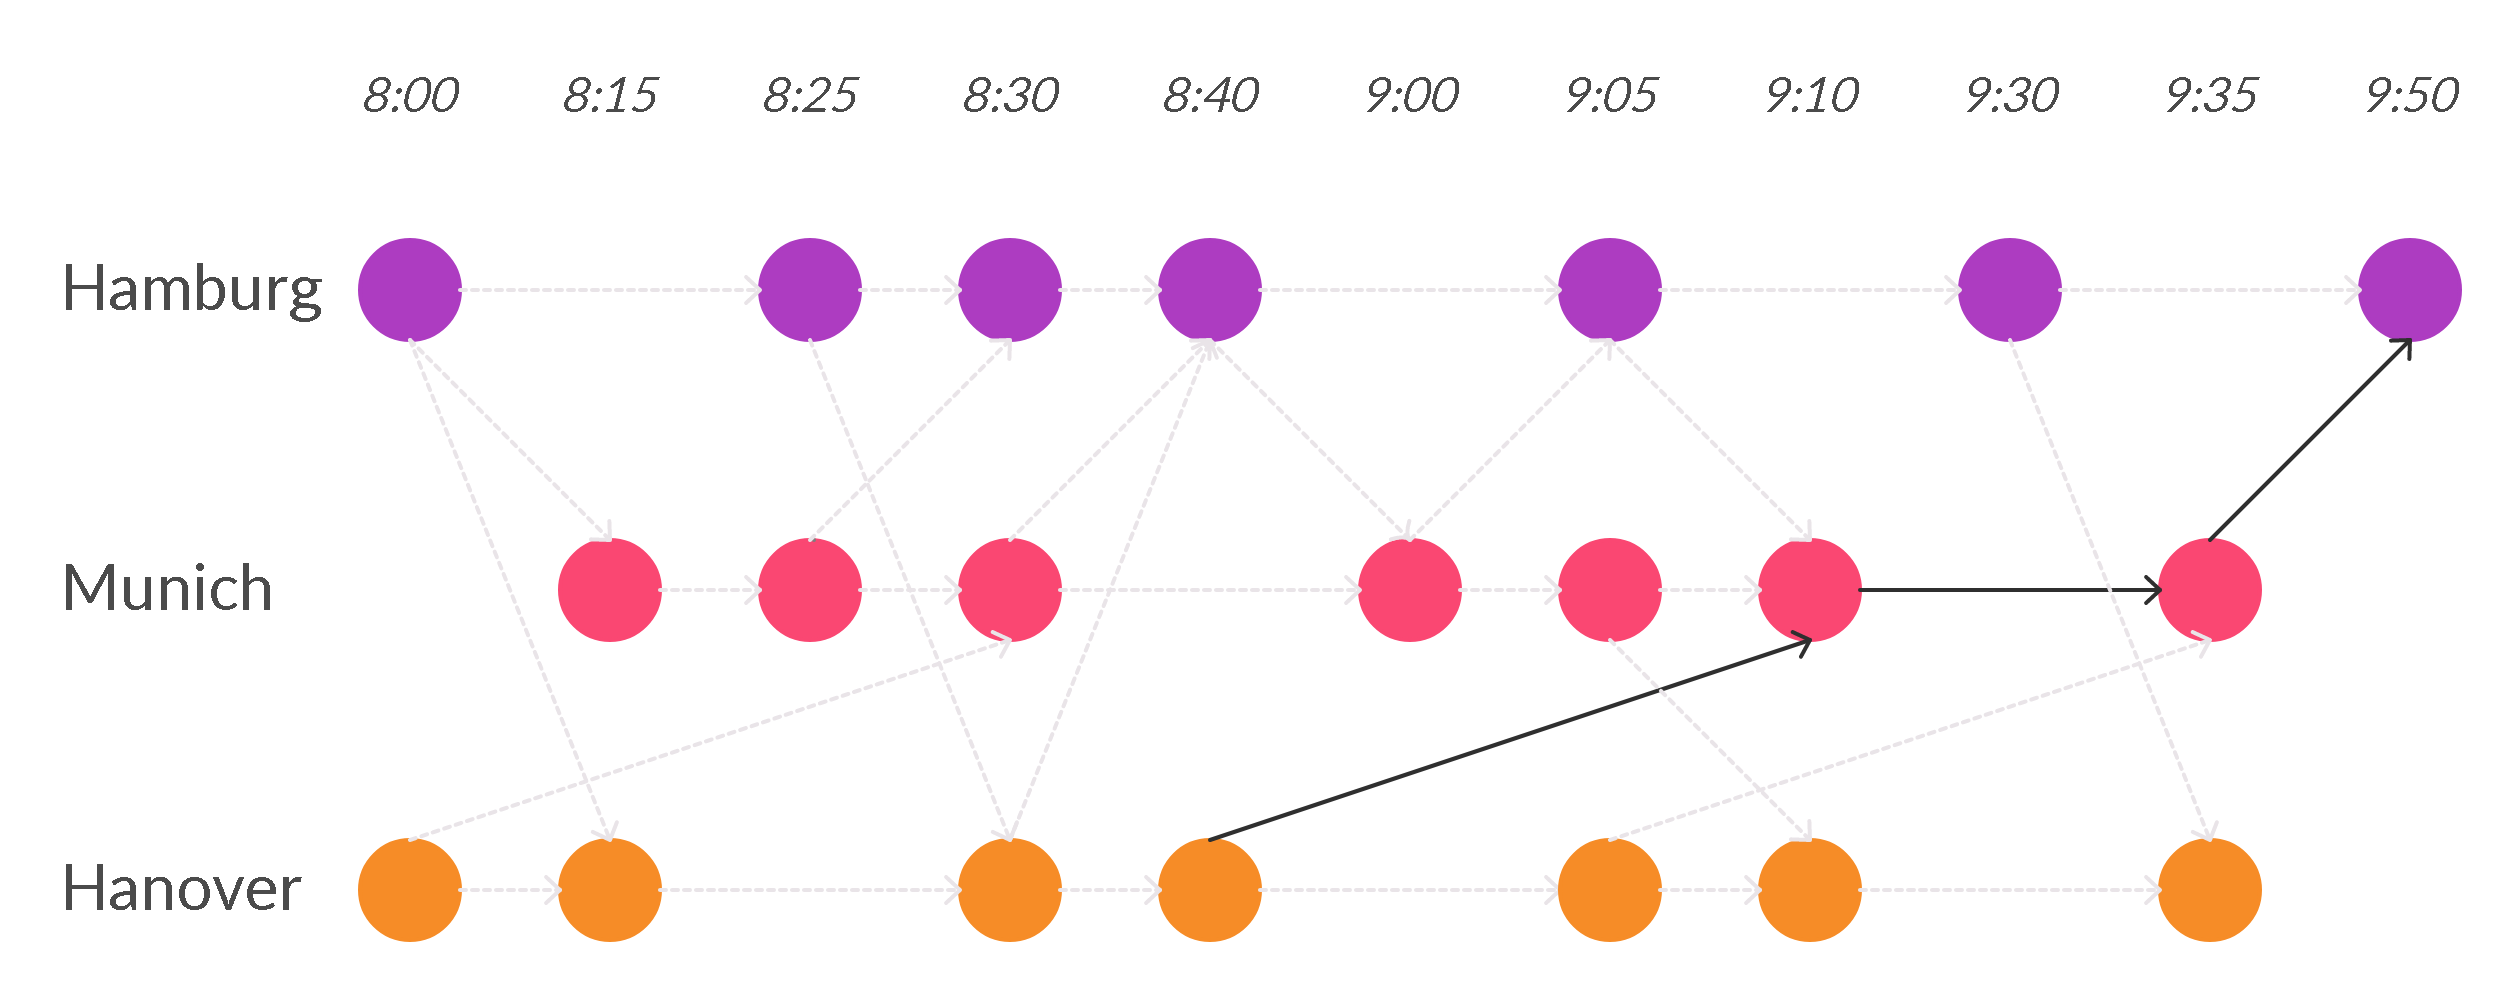
\includegraphics[scale=.15]{pics/Passenger_Path_Example.jpg}
%     \caption{Example of a trajectory taken by a passenger. Each path can be identified as a sequence of arcs. This depicts one $\lambda\in\Lambda$.}
%     \label{fig:passenger_path}
% \end{figure}
% \begin{figure}
%     \centering
%     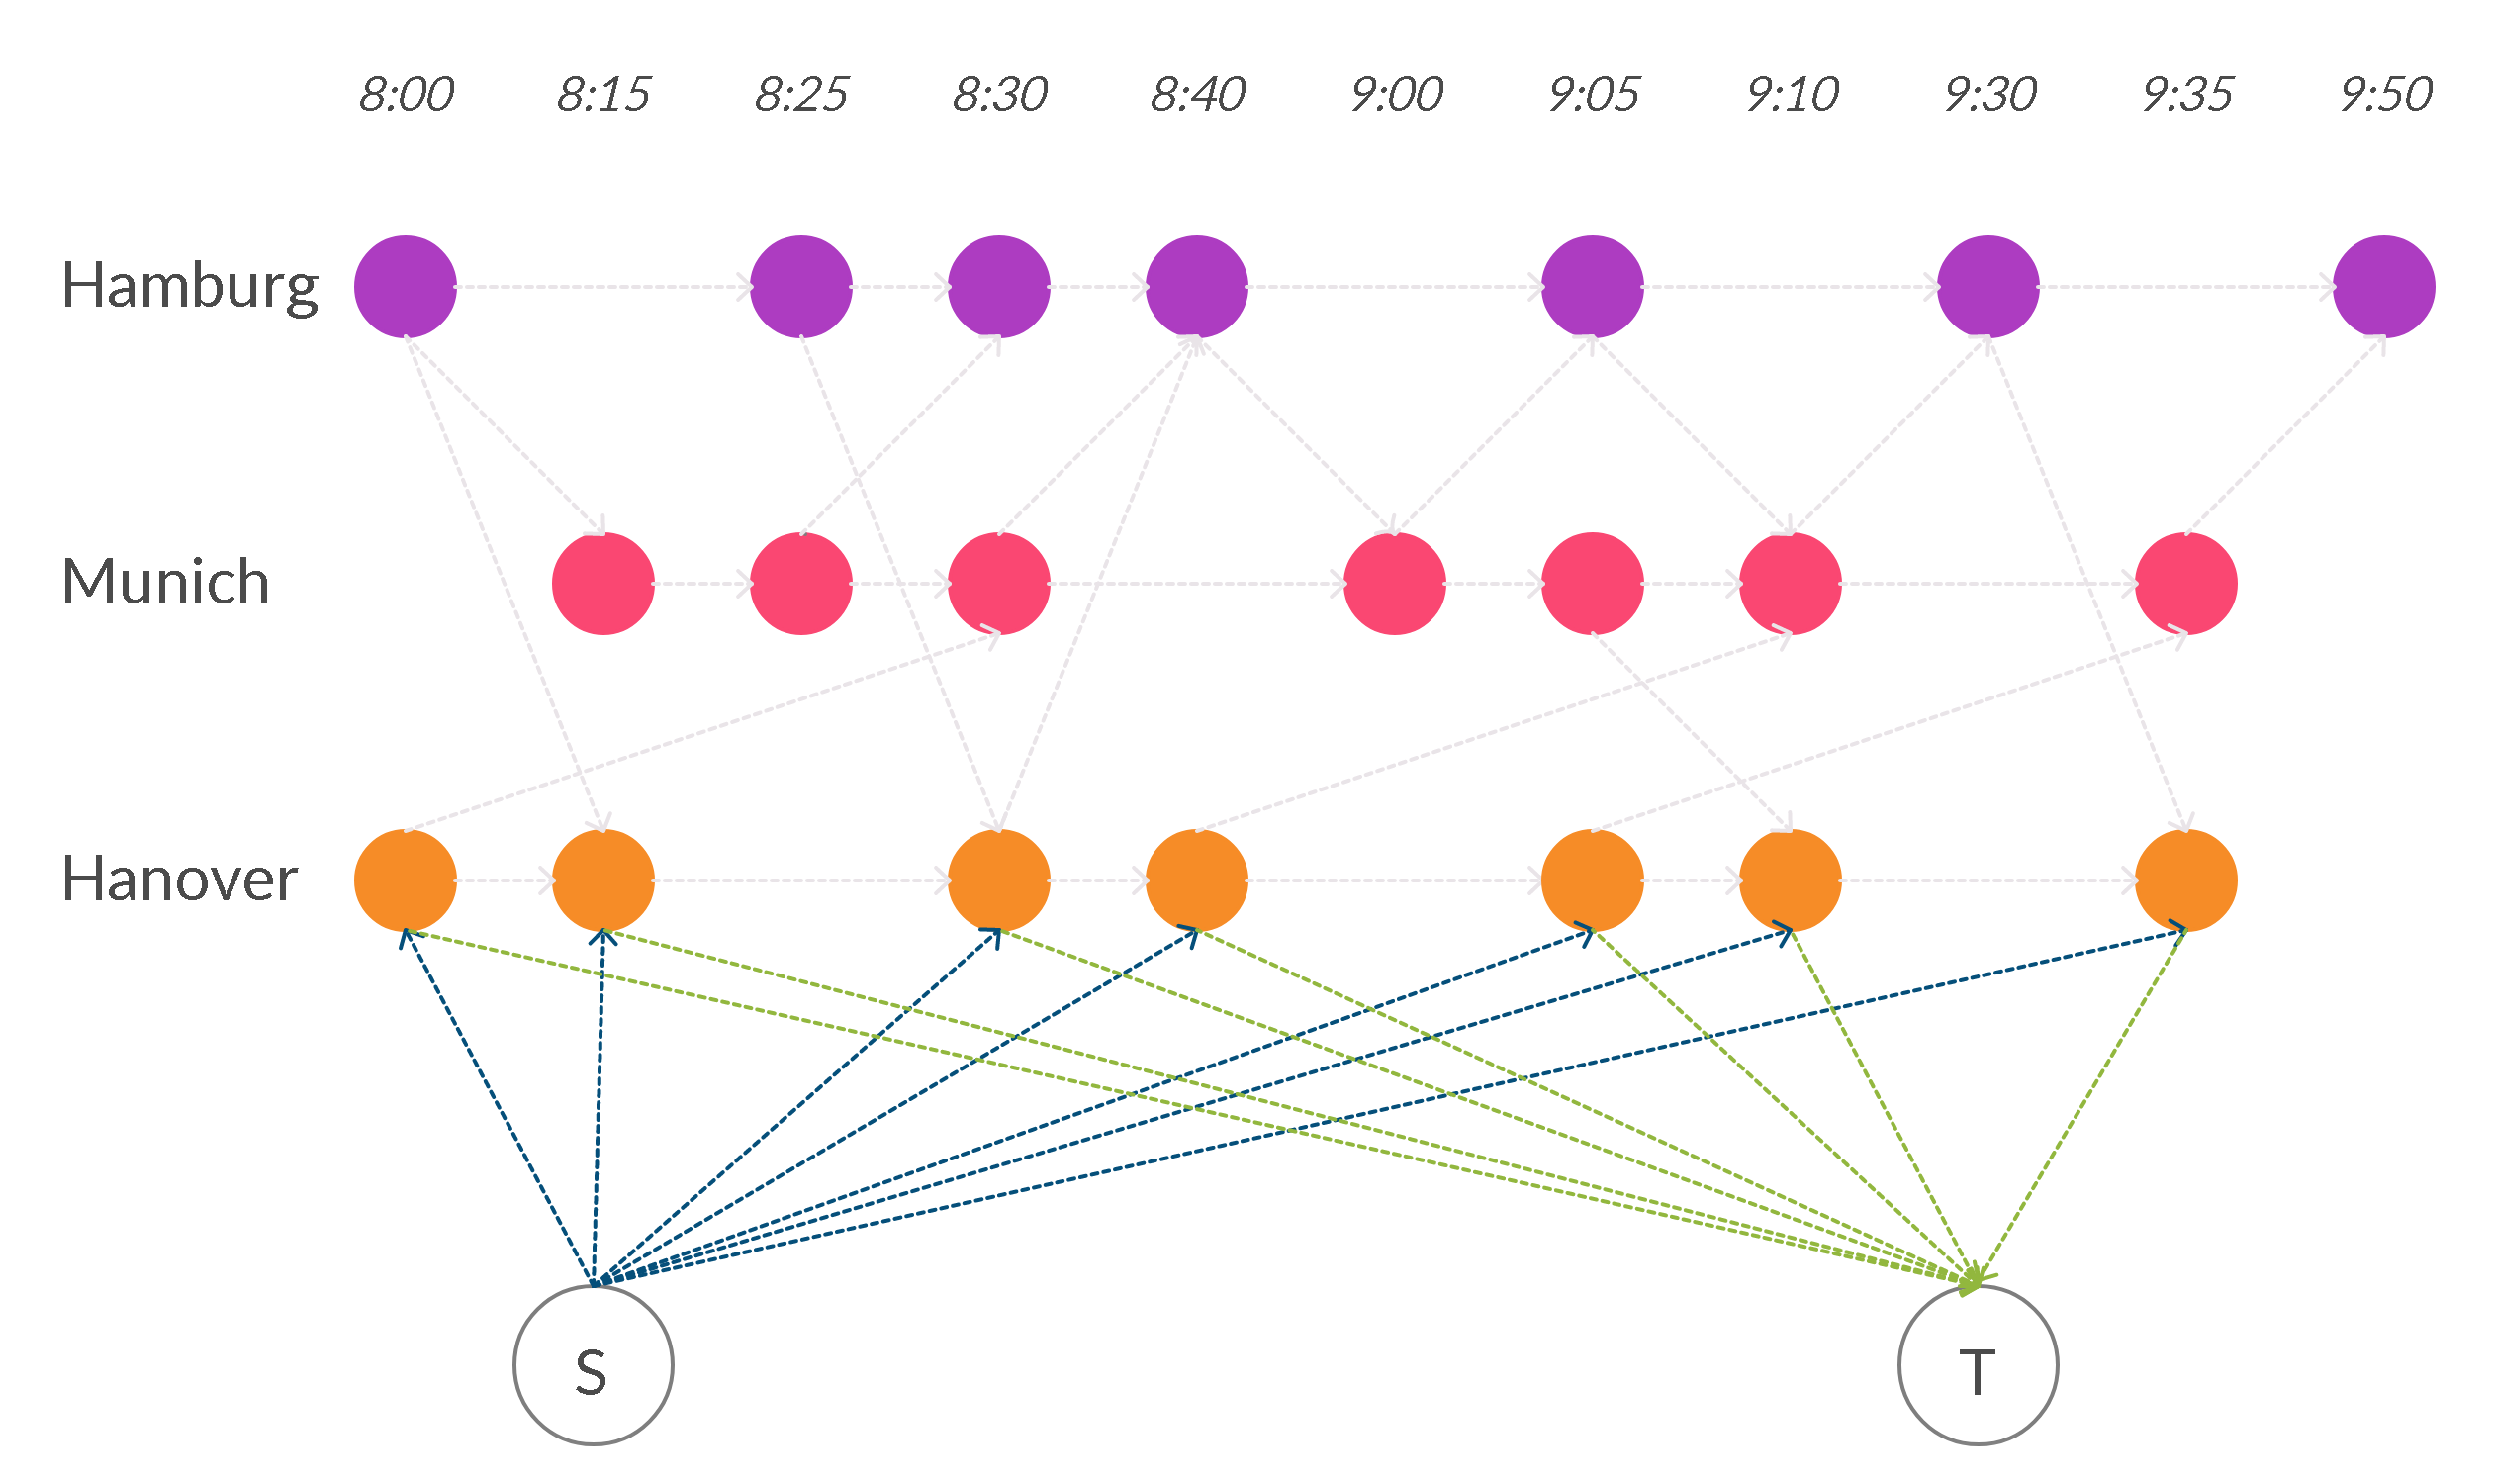
\includegraphics[scale=.15]{pics/Source_Sink_Edges.jpg}
%     \caption{Example graph including dummy nodes called source and sink which are fully connected to all nodes of the Hanover station.}
%     \label{fig:sink_and_source}
% \end{figure}
% \begin{figure}
%     \centering
%     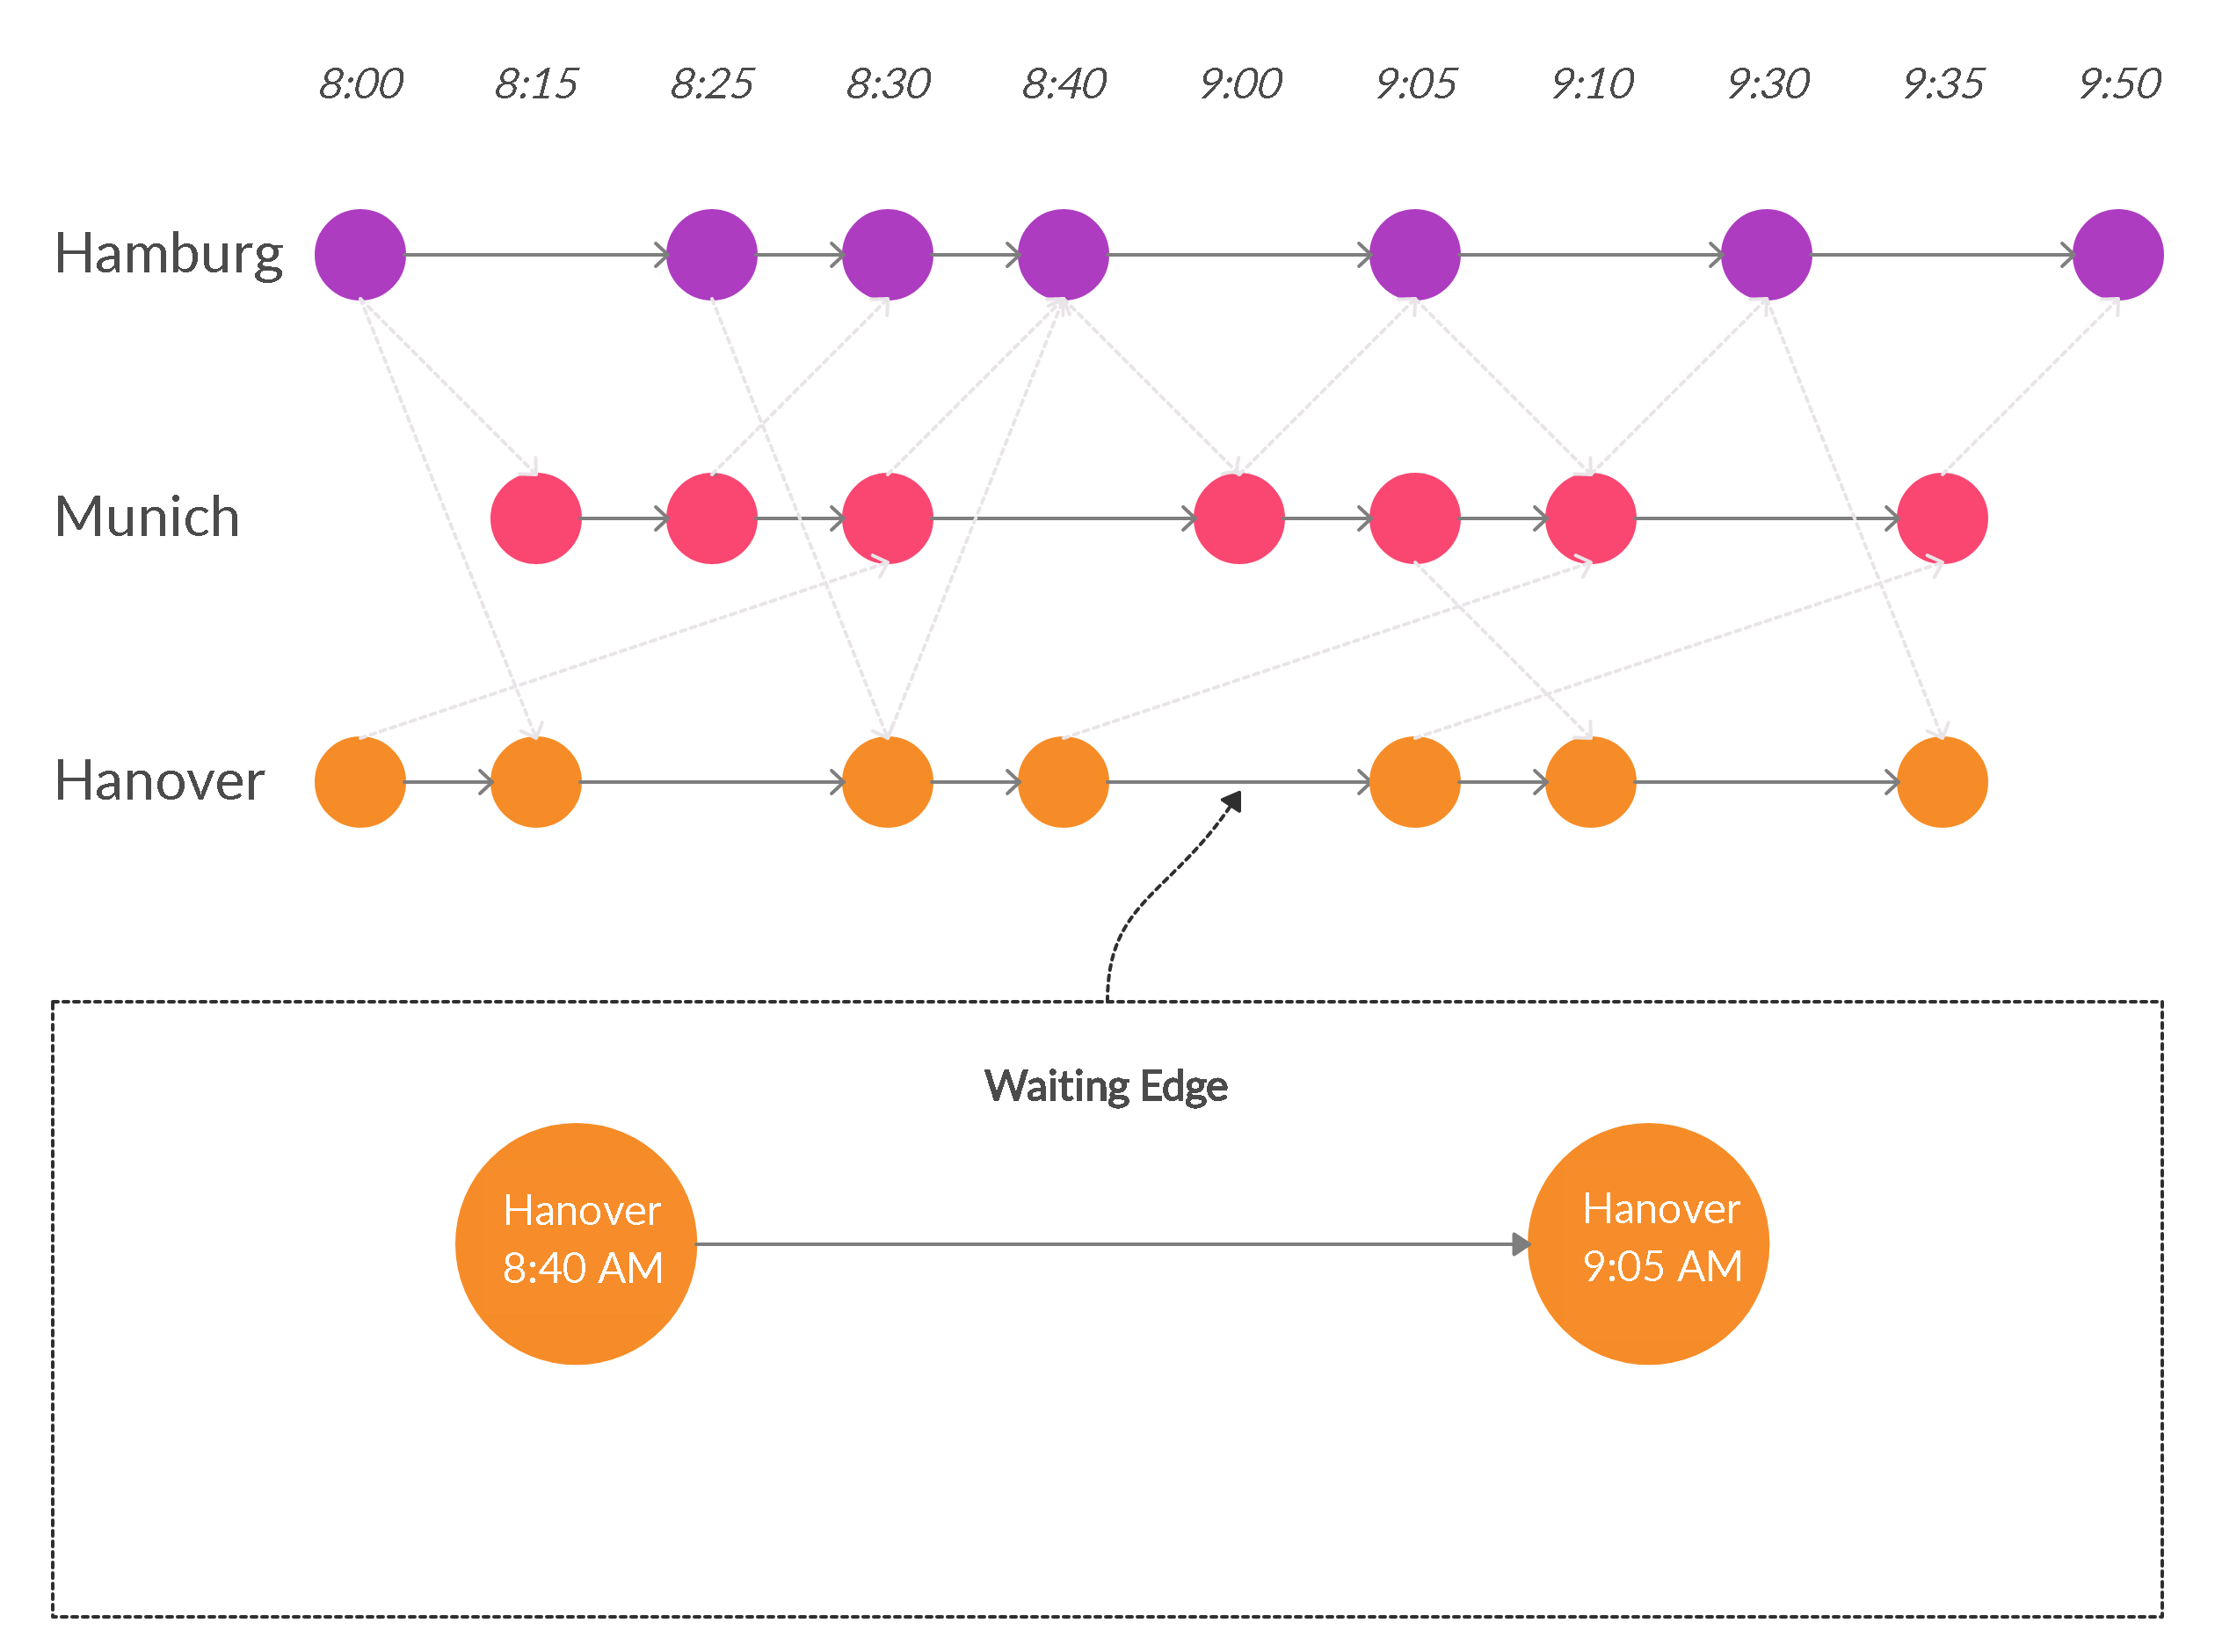
\includegraphics[scale=0.15]{pics/Waiting_Edges.jpg}
%     \caption{Example graph depicting only the waiting arcs.}
%     \label{fig:waiting_arcs}
% \end{figure}
% \end{appendix}


\bibliographystyle{model1-num-names}
\bibliography{references}
\end{document}